%%% Présentation de Beamer

\part{Beamer}

\section{Utilisation de Beamer}

\begin{frame}[fragile]
  \frametitle{Qu'est-ce que Beamer ?}

Beamer est une classe \LaTeX{} :

\lstinline?\documentclass{beamer}?

\medskip
Points communs :
\begin{itemize}
  \item \bemph{structuration} (parties, sections, sous-sections ; pas de chapitres),
  \item mise en forme du texte,
  \item inclusion de \bemph{figures} et de \bemph{formules mathématiques},
  \item etc.
\end{itemize}

\medskip
Différences :
\begin{itemize}
  \item structuration en \bemph{diapositives},
  \item nouvelles commandes (\bemph{transitions}/animations),
  \item mise en page différente (police, agencement).
\end{itemize}
\end{frame}



\begin{frame}[fragile]
  \frametitle{Définition du document}

Beamer est une classe \LaTeX{} :

\lstinline?\documentclass[options]{beamer}?

\medskip
Parmi les \lstinline?options? :
\begin{itemize}
  \item \lstinline?t?, \lstinline?c? ou \lstinline?b? pour aligner verticalement le texte en haut, au milieu ou en bas de la diapositive,
  \item \lstinline?Xpt? pour définir la taille de la police à \lstinline?X? (ex : \lstinline?9pt?),
  \item \lstinline?handout? pour obtenir une version imprimable (sans transitions/animations).
\end{itemize}

\medskip
Puis le préambule, et le contenu du document dans :
\begin{lstlisting}
\begin{document}
  ...
  ...    % Les diapositives ici
  ...
\end{document}
\end{lstlisting}
\end{frame}



\begin{frame}[fragile]
  \frametitle{Définition d'une diapositive}

Chaque diapositive est comprise dans un environnement \lstinline?frame? :

\begin{lstlisting}
 \begin{frame}[options]
   ...
   ...    % Contenu de la diapositive
   ...
 \end{frame}
\end{lstlisting}

\medskip
Les \lstinline?options? peuvent contenir :
\begin{itemize}
  \item \lstinline?t?, \lstinline?c? ou \lstinline?b? pour changer l'alignement vertical du texte pour cette diapositive uniquement,
  \item \lstinline?plain? pour ne pas afficher les bandeaux d'en-tête et de pied pour cette diapositive,
  \item \lstinline?shrink? pour tasser le texte s'il y en a beaucoup,
  \item \lstinline?fragile? si la diapositive contient du code (comme ici).
\end{itemize}
\end{frame}



\begin{frame}[fragile]
  \frametitle{Propriétés d'une diapositive}
  \framesubtitle{Titre, sous-titre et bandeaux}

On peut définir un titre et un sous-titre pour une diapositive :

\begin{lstlisting}
\frametitle{£\meta{Titre de la diapo}£}
\framesubtitle{£\meta{Sous-titre de la diapo}£}
\end{lstlisting}

\bigskip
De plus, selon le thème, des informations s'affichent dans les bandeaux d'en-tête et de pied :
\begin{itemize}
  \item section en cours,
  \item titre de la présentation, date, nom des auteurs et institut,
  \item numérotation des diapositives.
\end{itemize}
\end{frame}



\begin{frame}[fragile]
  \frametitle{À l'intérieur d'une diapositive}

Le contenu d'une diapositive est du \LaTeX{} habituel :
\begin{itemize}
  \item listes,
  \item figures (contenant tableaux, figures complexes, images...),
  \item texte et équations mathématiques,
  \item etc.
\end{itemize}

\medskip
On peut aussi englober ces éléments dans des blocs :
\begin{lstlisting}
\begin{exampleblock}{Titre du bloc}
  Contenu du bloc (listes, £\'e£quations, maths, ...)
\end{exampleblock}
\end{lstlisting}

\begin{exampleblock}{Titre du bloc}
  Contenu du bloc (listes, équations, maths, ...)
\end{exampleblock}

\medskip
3 types de blocs : \lstinline?block?, \lstinline?alertblock? et \lstinline?exampleblock?.
\end{frame}



\begin{frame}[plain]
\begin{figure}
  \centering
  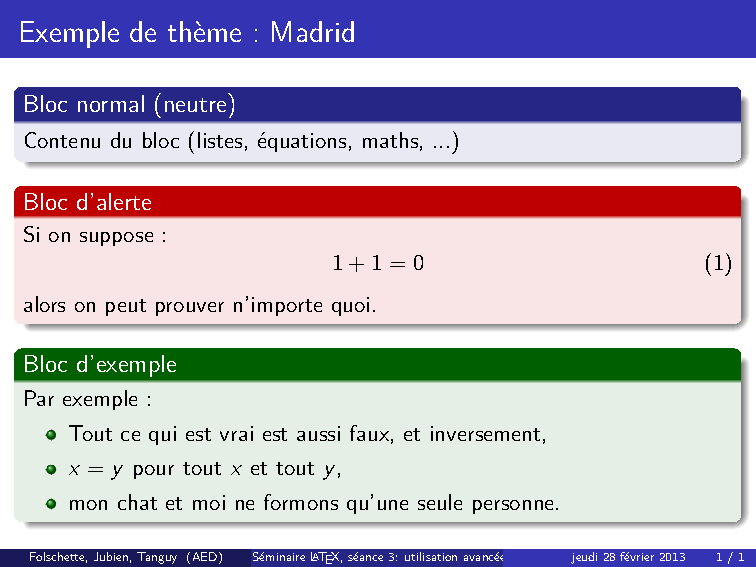
\includegraphics[width=1\textwidth]{img/seance3_extheme_madrid}
\end{figure}
\end{frame}



\section{Les animations en Beamer}

\begin{frame}[fragile]
  \frametitle{Animations}

On peut définir des animations (statiques) au sein des présentations.
\begin{itemize}
  \item<2,4-> Elles consistent en des apparitions...
  \item<3-> ...ou des disparitions.
\end{itemize}

\bigskip
\pause[4]
Les animations créent plusieurs pages pour la même diapositive, avec les différences nécessaires. La numérotation n'est pas affectée.

\medskip
L'option \lstinline?handout? du \lstinline?\documentclass? permet de supprimer ou de simplifier ces animations.
\end{frame}



\begin{frame}[fragile]
  \frametitle{Apparitions successives}

Avec la commande \lstinline?\pause? ou \lstinline?\pause[x]?

\medskip
Exemple avec \lstinline?\pause? :

\begin{columns}
  \begin{column}{0.20\textwidth}
\begin{lstlisting}
| Texte 1,
| \pause
| Texte 2,
| \pause
| Texte 3,
| \pause
| Texte 4.
\end{lstlisting}
  \end{column}
  \begin{column}{0.35\textwidth}
\myex{
Texte 1,
\pause
Texte 2,
\pause
Texte 3,
\pause
Texte 4.
}
  \end{column}
\end{columns}
\end{frame}



\begin{frame}[fragile]
  \frametitle{Animations avancées}

Deux commandes :
\begin{itemize}
  \item \lstinline?\only<pages>{contenu}? dévoile \lstinline?contenu? \bemph{uniquement} dans les \lstinline?pages? spécifiées,
  \item \lstinline?\uncover<pages>{contenu}? fait de même, mais \bemph{réserve l'espace} non occupé lorsqu'il n'est pas affiché.
\end{itemize}

Le \lstinline?contenu? peut être n'importe quoi (texte, figures, mathématiques, etc.).

\medskip
Les \lstinline?<pages>? sont définies par groupes :
\begin{itemize}
  \item \lstinline?<n>? : la page $n$,
  \item \lstinline?<-n>? : toutes les pages avant $n$ compris,
  \item \lstinline?<n->? : toutes les pages à partir de $n$,
  \item \lstinline?<n-p>? : toutes les pages entre $n$ et $p$ inclus,
  \item \lstinline?<x,y>? : le groupe de pages $x$ et le groupe de pages $y$.
\end{itemize}
\end{frame}



\begin{frame}[fragile]
  \frametitle{Animations avancées}

Exemple avec \lstinline?\only? :
\begin{columns}
  \begin{column}{0.40\textwidth}
\begin{lstlisting}
| Texte 1,
| 
| \only<2->{Texte 2 qui appara£\^{i}£t,}
| 
| Texte 3.
\end{lstlisting}
  \end{column}
  \begin{column}{0.37\textwidth}
\myex{
Texte 1,

\only<2->{Texte 2 qui appara\^{i}t,}

Texte 3.
}
  \end{column}
\end{columns}

\bigskip
Exemple avec \lstinline?\uncover? :
\begin{columns}
  \begin{column}{0.40\textwidth}
\begin{lstlisting}
| Texte 1,
| 
| \uncover<3->{Texte 2 qui appara£\^{i}£t,}
| 
| Texte 3.
\end{lstlisting}
  \end{column}
  \begin{column}{0.37\textwidth}
\myex{
Texte 1,

\uncover<3->{Texte 2 qui appara\^{i}t,}

Texte 3.
}
  \end{column}
\end{columns}

\end{frame}



\begin{frame}[fragile]
  \frametitle{Animations avancées}

D'autres commandes peuvent prendre un argument \lstinline?<pages>? optionnel.

\bigskip
Exemple : \lstinline?\item<pages>?
\begin{columns}
  \begin{column}{0.40\textwidth}
\begin{lstlisting}
\begin{itemize}
  \item<1,5> Premier £\'e£l£\'e£ment
  \item<2,4-> Second £\'e£l£\'e£ment
  \item<3-> Troisi£\`e£me £\'e£l£\'e£ment
\end{itemize}\end{lstlisting}
  \end{column}
  \begin{column}{0.40\textwidth}
\myex{
\begin{itemize}
  \item<1,5> Premier élément
  \item<2,4-> Second élément
  \item<3-> Troisième élément
\end{itemize}
}
  \end{column}
\end{columns}

\pause[5]
\end{frame}



\begin{frame}[fragile, t]
  \frametitle{Animations TikZ}

\begin{figure}
  \begin{tikzpicture}
    \tikzexnodes
    \tikzexedges
\node<2> at (rond) [rectangle, fill=green!20, draw, thick] {Oui !} ;
\node<3> at (ellipse) [rectangle, fill=red!20, draw, thick] {Non !} ;
  \end{tikzpicture}
\end{figure}

\bigskip
Beaucoup de commandes TikZ acceptent aussi la syntaxe \lstinline?<pages>? pour créer des animations dans une présentation.

\bigskip
\begin{lstlisting}
\node<2> at (rond) [square, fill=green!20, draw, thick] {Oui !} ;
\node<3> at (ellipse) [square, fill=red!20, draw, thick] {Non !} ;
\end{lstlisting}
\end{frame}



\section{Personnalisation de Beamer}

\begin{frame}[fragile]
  \frametitle{Les thèmes}

Il est possible d'utiliser des thèmes prédéfinis pour modifier l'apparence et les couleurs d'une présentation. On peut spécifier :
\begin{itemize}
  \item Un \bemph{thème d'agencement} avec \lstinline?\usetheme{theme}? :
  \begin{itemize}
    \item style de la page de titre et agencement des diapos,
    \item forme et contenu des bandeaux,
    \item police, forme des puces, ...
  \end{itemize}
  Exemples : \lstinline?Warsaw?, \lstinline?Madrid?, \lstinline?Copenhagen?, \lstinline?CambridgeUS?...
  \item Un \bemph{thème de couleurs} avec \lstinline?\usecolortheme{theme}? :
  \begin{itemize}
    \item couleur du texte, des titres, du sommaire,
    \item couleur de fond, des blocs, des bandeaux...
  \end{itemize}
  Exemples : \lstinline?beaver?, \lstinline?dolphin?, \lstinline?dove?, \lstinline?fly?...
\end{itemize}

\bigskip
Pour une liste des thèmes par défaut, voir le WikiBooks \cite{wikibooksbeamer}.
\end{frame}



\begin{frame}[fragile]
  \frametitle{Personnaliser un thème}

Il est aussi possible de personnaliser en partie un thème ou de créer un thème, pour :
\begin{itemize}
  \item modifier le contenu des bandeaux d'en-tête et de pied,
  \item revoir l'agencement,
  \item supprimer des éléments inutiles (sommaire, icônes...),
  \item adapter certaines couleurs.
\end{itemize}

\bigskip
On peut pour cela redéfinir toutes les caractéristiques d'une présentation :
\begin{itemize}
  \item les agencements,
  \item les couleurs.
\end{itemize}

\bigskip
Pour une liste des options modifiables, voir le WikiBooks \cite{wikibooksbeamer}.
\end{frame}



\subsection{Exemples}

\begin{frame}[fragile]
  \frametitle{Exemple de thème : CambridgeUS}

\begin{block}{Bloc normal (neutre)}
  Contenu du bloc (listes, équations, maths, ...)
\end{block}

\begin{alertblock}{Bloc d'alerte}
  Si on suppose :
  \begin{equation}
    1+1=0
  \end{equation}
  alors on peut prouver n'importe quoi.
\end{alertblock}

\begin{exampleblock}{Bloc d'exemple}
  Par exemple :
  \begin{itemize}
    \item Tout ce qui est vrai est aussi faux, et inversement,
    \item $x = y$ pour tout $x$ et tout $y$,
    \item mon chat et moi ne formons qu'une seule personne.
  \end{itemize}
\end{exampleblock}
\end{frame}



\begin{frame}[plain]
\begin{figure}
  \centering
  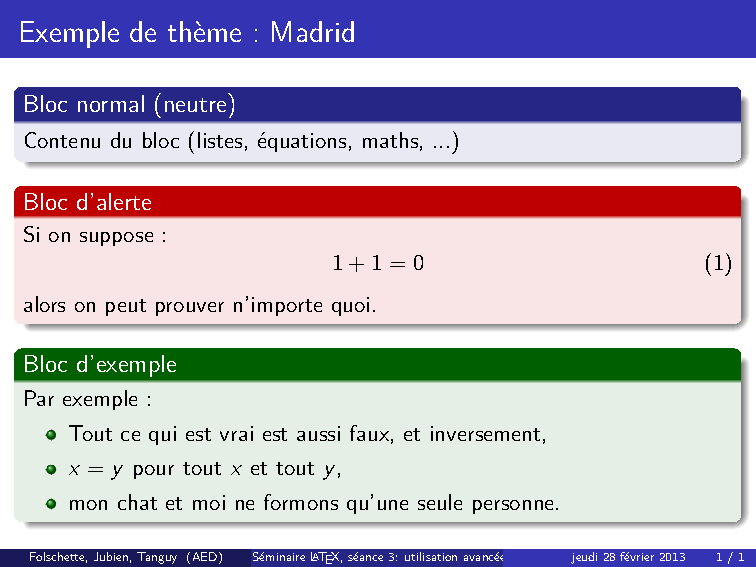
\includegraphics[width=1\textwidth]{img/seance3_extheme_madrid}
\end{figure}
\end{frame}



\begin{frame}[plain]
\begin{figure}
  \centering
  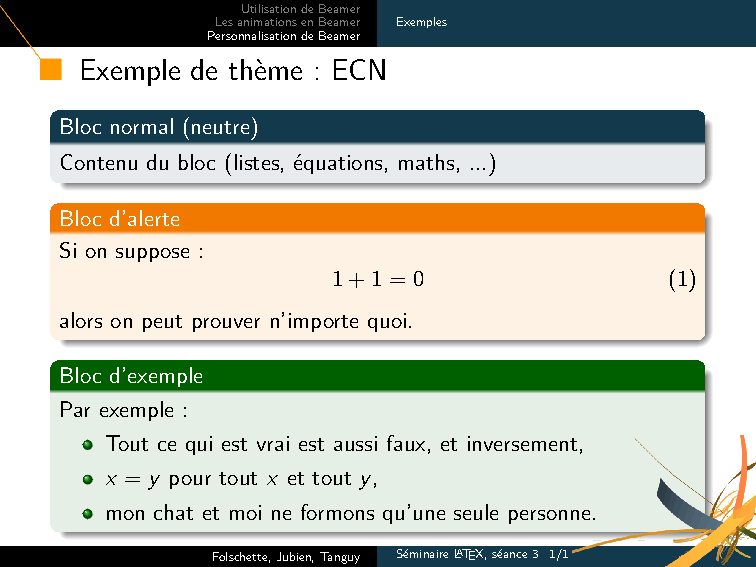
\includegraphics[width=1\textwidth]{img/seance3_extheme_ecn}
\end{figure}
\end{frame}



\begin{frame}[plain]
\begin{figure}
  \centering
  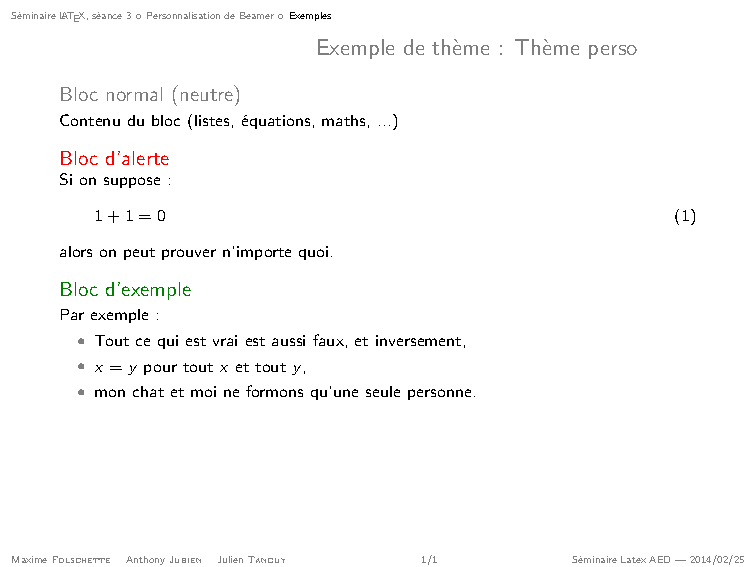
\includegraphics[width=1\textwidth]{img/seance3_extheme_perso}
\end{figure}
\end{frame}



\subsection{Exercice}

\begin{frame}[fragile]
  \frametitle{Exercice}

Une présentation simple :

\begin{lstlisting}[multicols=2]
  \documentclass{beamer}

  \usepackage[french]{babel}
  \usepackage[utf8]{inputenc}

  \usetheme{Madrid}
  \usecolortheme{default}

  \title{Pr£\'e£sentation de ma th£\`e£se}
  \author{Pr£\'e£nom Nom}
  \institute[LDC]{Laboratoire des Chatons}

  \begin{document}

  \begin{frame}
    \maketitle
  \end{frame}

  % A partir d'ici,
  % entrez ce que vous voulez...
  \section{£\`A£ propos de moi}

  \begin{frame}
    \frametitle{Ce que j'aime}
    \begin{itemize}
      \item Les chatons,
      \pause
      \item le jus de raisin,
      \pause
      \item etc.
    \end{itemize}
  \end{frame}

  \end{document}
\end{lstlisting}

\end{frame}


